\documentclass[10pt]{IEEEtran}
\title{Exploring Protocol Layers with Wireshark}
\author{Lucas Enloe, Vivek Pahwa}
\usepackage{graphicx}
\makeatletter
\newcommand{\rmnum}[1]{\romannumeral #1}
\newcommand{\Rmnum}[1]{\expandafter\@slowromancap\romannumeral #1@}
\makeatother
\usepackage{cite}
\usepackage{flushend}
\begin{document}

\maketitle

\begin{abstract}
Wireshark is a popular open-source program that allows users to capture and analyze network traffic. A useful property of Wireshark is that it allows the user to break down network traffic into component protocols and study the protocols individually. By completing Wireshark labs, we gain increased familiarity with the Wireshark software by investigating a number of common network protocols. Additionally, we gain an increased understanding of individual protocols by observing and analyzing them in a hands-on, real-world environment.
\end{abstract}

\section{Introduction}
\IEEEPARstart{W}{ireshark} is used for protocol development, network troubleshooting, and packet analysis \cite{wireshark}. It helps capture different networking protocols which are generated from various sources such as Ethernet, IEEE 802.11, NetSim, OPNET, and ns. The captured packets are displayed to the user in a color coded scheme depending on the type of traffic and are accessed, either using the GUI or the command line. In this project, we have utilized this tool to capture and analyze six important upper layer protocols, namely, HTTP, IP, ICMP, DHCP, UDP and TCP.

 Internet Protocol (IP) is a layer three protocol in the OSI protocol suite and enables internetworking by routing and forwarding packets. ICMP works above IP but is still a layer three protocol. It is used to report errors such as source quenching or time exceeded and provide operational services such as issuing an ECHO request/response query or an address mask request/response query. TCP and UDP are transport layer protocols that provide process to process communication. TCP is a reliable, connection-oriented protocol, whereas UDP provides unreliable and connectionless service. Both protocols have distinct uses: FTP and telnet are done using TCP, for example, while real time media streaming is done using UDP. DHCP and HTTP work on the application layer of the protocol stack. DHCP dynamically provides a user with the network configuration parameters required to join a network. HTTP is an application layer protocol which runs over TCP and defines how files are sent over the world wide web \cite{tanenbaum}
 
 The rest of the paper is organized as follows. In Section \Rmnum{2} to \Rmnum{7}, labs corresponding to each of the aforementioned protocols are performed. Each of the lab provides an overview about the functioning of the individual protocol and is a comprehensive answer to the tasks mentioned in the labs. Finally, the conclusion is drawn in Section \Rmnum{8}.\\ 

\section{Lab 1: Introduction to Wireshark}

 The goal of the first lab is to familiarize the user with the Wireshark packet analysis tool, and to explore some of its capabilities. The lab takes a bottom to top approach and guides the user from setting up and running Wireshark on the host machine to working on it and understanding its functionalities. The Wireshark interface has five major components: (1)  Command menus are pulldown menus which are located at the top of the window. It includes the capture menu, which allows the user to begin packet capture. (2) The Packet-Listing window provides a one-line summary of each captured packet including details like source and destination address, protocol type, and protocol specific information contained in the packet. (3) The Packet-Header details window provides information about the selected packet, including the Ethernet frame, IP datagram, and layer 4 segment. We can view fields of all the headers added to an upper layer data. (4) The Packet-Contents window displays the contents of the captured frame in both ASCII and hexadecimal format. (5) The Packet Display Filter field filters out the captured packets based on the data entered. Packets can be filtered by a wide variety of properties.
 
 The functionalities of Wireshark are tested by capturing packets while exchanging HTTP messages with the \textit{gaia.cs.umass.edu} server in order to download the page content. The captured packets are displayed in the Packet-Listing window. These packets contain various types of protocols such as DNS, TCP, ARP, HTTP, and SSDP to name a few. After filtering out the HTTP messages from the captured packets, we can obtain a myriad of information about the communication that took place between the two machines. It takes around 45ms to receive a HTTP OK message in response to a HTTP GET message sent out by the host machine. We can obtain the IP address of the server as well as the host machine, which is 128.119.245.12 and 192.168.0.7, respectively. The fact that HTTP works above the TCP can be verified by looking at the transport layer segment . Figure \ref{fig:HTTPpacket} shows a captured HTTP GET message sent out from our machine to the server.  \\

\begin{figure}[h!]
	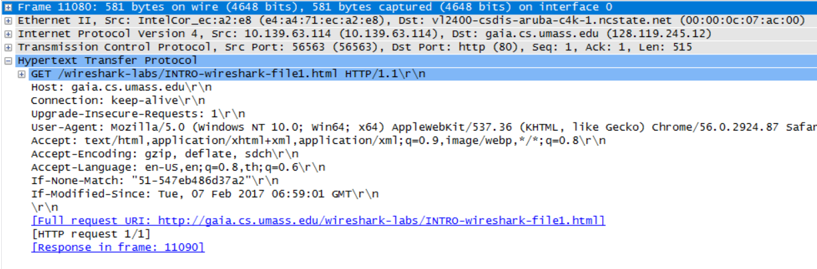
\includegraphics[width=\linewidth]{HTTP_GET.png}
	\caption{Captured HTTP GET packet}
	\label{fig:HTTPpacket}
\end{figure}

\section{Lab 2: The Internet Protocol Datagram}

 The purpose of Lab 2 is to investigate the Internet Protocol (IP), specifically the IP datagram. This is accomplished by capturing and analyzing packets from executions of the {\tt traceroute} command. The {\tt traceroute} program sends datagrams with incrementing time-to-live (TTL) values, starting with 1 and increasing until the final destination or maximum TTL value is reached. Routers reduce the TTL of every received packet by 1, and if the TTL is 0 after decrementing, the router drops the packet at sends an ICMP TTL-exceeded message to the original sender of the packet. By sending packets with incrementing TTL values, the {\tt traceroute} program can identify individual hop points between the sender and the destination by compiling all the TTL-exceeded messages received during execution of the program \cite{tanenbaum}
 
 We will capture packets obtained from a {\tt traceroute} to the IEEE Information Theory Society website: www.itsoc.org. We will use the Ping Plotter software on Windows, which allows us to adjust the size of the datagrams. Three separate traces are conducted, using datagram lengths of 56, 2000, and 35000 bytes. Figure \ref{fig:packet1} shows a captured IP datagram sent from our computer during the execution of a {\tt traceroute} with 56 byte packets. The traceroute itself, as well as additional packets, can be found in Appendix A.\\
 
\begin{figure}[h!]
	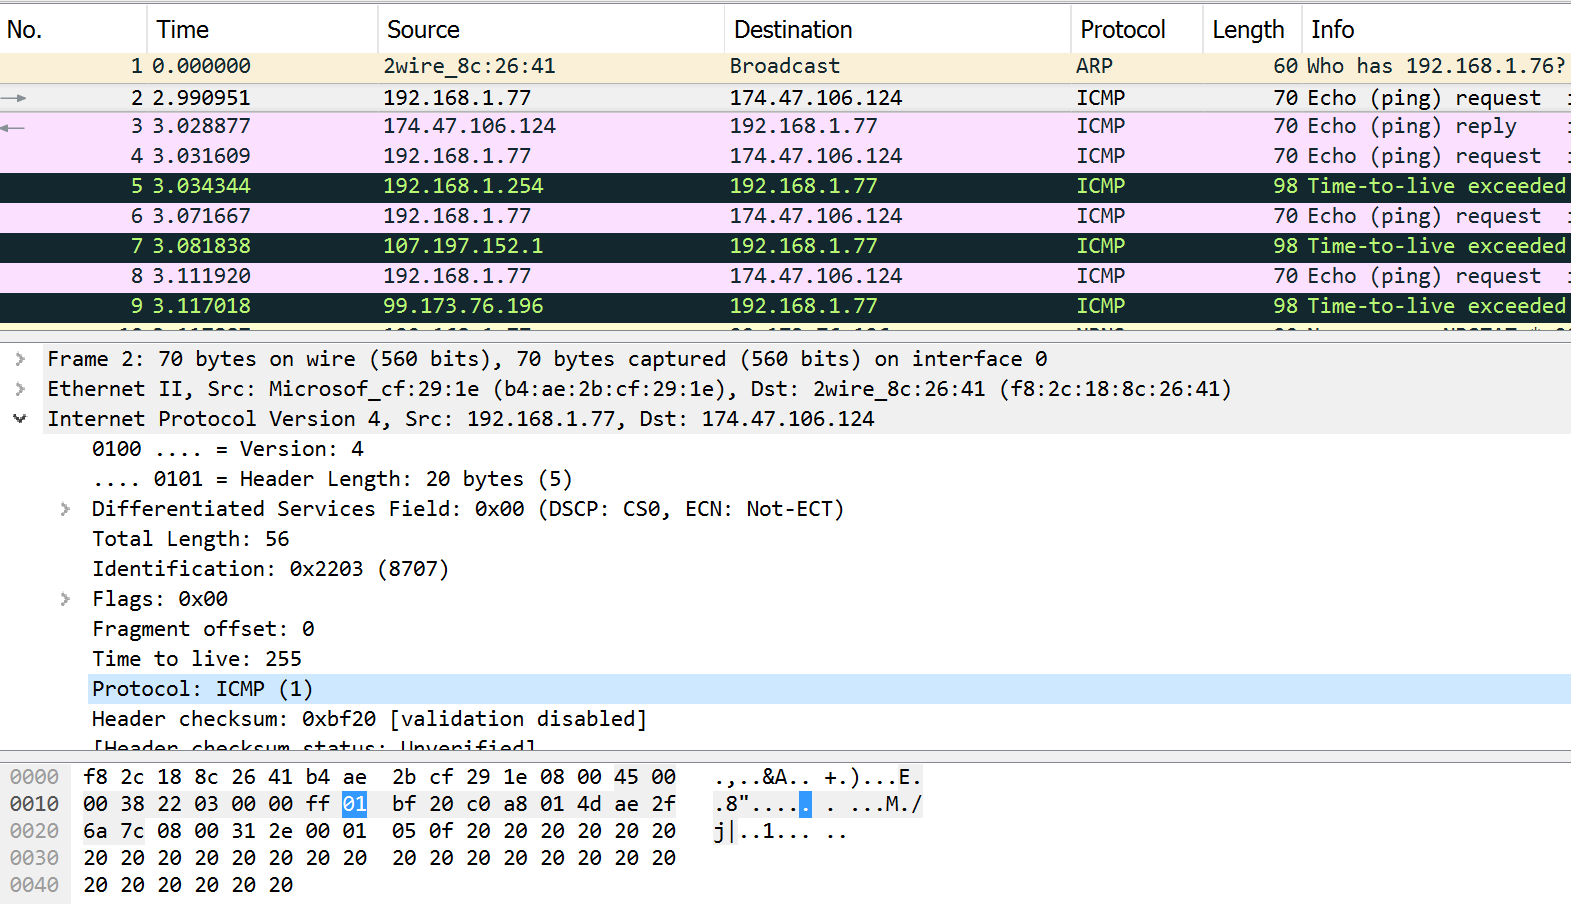
\includegraphics[width=\linewidth]{lab2packet1.png}
	\caption{Captured 56 byte IP Datagram}
	\label{fig:packet1}
\end{figure}
 
 Several key details can be gleaned from the Internet Protocol section of the ICMP Echo Request message. For example, in this execution, the IP address of the requesting source, our computer, is 192.168.1.77. The Protocol Field value is 1, indicating an ICMP message. Other common values are 6 for TCP and 17 for UDP. The IP header contains 20 bytes, while the payload itself contains 36 bytes. We can verify payload size multiple ways. First, we know from our settings that the datagram is 56 bytes in total, so a 20 byte header requires a 36 byte payload. Additionally, the ICMP section of the message in Wireshark shows 1 byte used for the message type, 1 byte for message code, a 2 byte checksum, a 2 byte identifier value, a 2 byte sequence number, and 28 bytes of data, which gives us a total of 36 bytes. We know the datagram has not been fragmented in this case because the fragment flag is not set.
 
 By sorting captured packets by source, we can easily view successive IP datagrams sent from our computer. We see that the sequence number always changes from packet to packet, while the type and code remain constant. Because of the changing sequence number, the checksum changes as well. The type and code values must remain constant to properly identify the type of ICMP message being sent. Additionally, the sequence number must always change to ensure echo-request and echo-reply pairs can be matched, as well as to identify packets that might have been lost. The data field does not change from packet to packet, however this is not a strict requirement. Because {\tt traceroute} is only concerned with adjusting TTL values to identify hop points, the specific contents in the data field are largely irrelevant. In the first ICMP TTL-exceeded replies sent to the computer from our hops, we see that the ICMP identification field value matches the same field value of the ICMP request sent by our computer. The TTL of the reply is 64. Because the protocol specification (RFC 791) does not require a specific TTL value, different operating systems have different TTL values. Network scanning tools such as Nmap take advantage of this fact to identify possible operating systems of hosts on a network.
 
 When the datagram size was increased to 2000 bytes, the datagram was fragmented into two separate packets. The IP header has the More Fragments flag set, and the total frame length is only 1514 bytes, even though we specified a datagram length of 2000 bytes. The second fragment of the datagram has an identical IP identification field value, with an offset of 1480 bytes, which was the length of the data field in the first fragment. The IP header fields that change between fragment pairs are the total length, flags, and checksum. Further increasing the datagram size to 3500 bytes causes each datagram to be fragmented into 3 packets. The total length and More Fragments flag remain the same for the first to packets of each fragmented datagram, while the final packet of each triplet is of shorter length and does not have the More Fragments flag set.\\
 
 
\section{Lab 3: The Internet Control Message Protocol}

 The purpose of this lab is to become familiar with the Internet Control Message Protocol (ICMP) and to explore different aspects of the it, such as the query/response messages generated during multiple programs. The format and the contents of an ICMP message are also investigated. ICMP carries two types of messages: Error reporting and Query/Response messages. The latter of the two is generated by programs with specific purposes, such as a Ping program or a Traceroute program. In this lab, we only examine the packets which are generated by these two programs.
 
 A Ping program is a tool that allows a user to check if a destination can be reached over the network. It is also used to check whether the destination machine is live. To achieve this, the source host sends a packet to the destination IP address. If the destination machine is reachable and live, the Ping program in the destination machine responds to the source machine by sending an ICMP packet back. In a Windows operating system, the command used to send out echo requests is, {\tt ping -n 10 hostname} in the MS-DOS command line. The argument {\tt -n 10} indicates that 10 ping messages should be sent and this value can be set to any desired number. For each response message, the source calculates the round-trip time (RTT) and displays the minimum, maximum and the average values of it. Out of the total packets sent, the number of packets which are lost is also displayed in the command line, as shown in the appendix. 
 
 Figure \ref{fig:pingRequest} shows the captured Echo request message sent from a machine with source IP address 10.139.62.77 to the destination with IP address 143.89.14.2. An ICMP message with type 8 and code 0 indicates an Echo request, whereas type 0 and code 0 indicates an Echo response. Although an ICMP message works above the IP layer in the protocol stack, it lacks source and destination port fields in its message format, as it is not a transport layer protocol. Aside from a Type and Code field, an ICMP message has the following fields present: Checksum, Identifier, Sequence Number, and Data. \\

\begin{figure}[h!]
	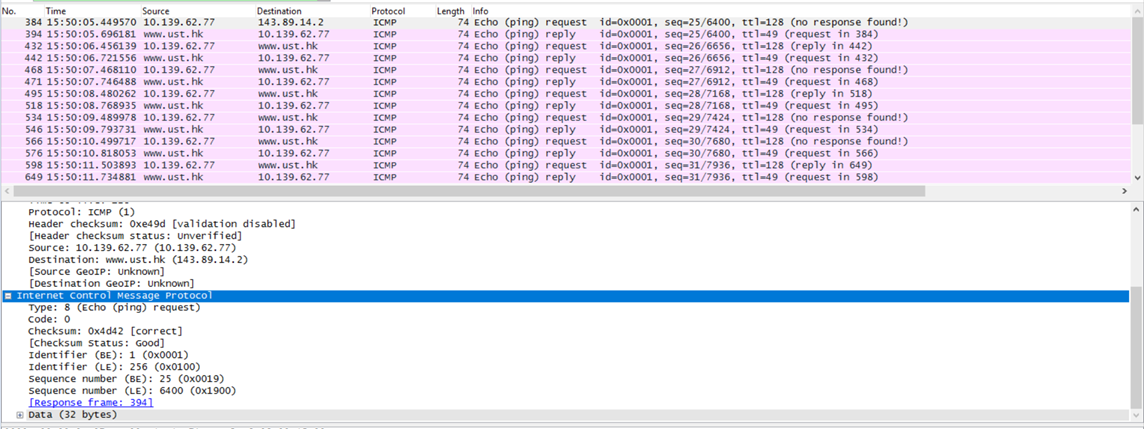
\includegraphics[width=\linewidth]{Echo_request.png}
	\caption{Captured ICMP Ping Query Message}
	\label{fig:pingRequest}
\end{figure}

 In Lab 2, we saw noted that when a packet's TTL reaches 0, a router sends a TTL Exceeded message back to the source of the packet. We will now go into further detail regarding the ICMP messages used during a Traceroute. An ICMP Echo message sent out during a Traceroute program is exactly same as the Echo message sent during a Ping program. So, the type and code fields have the same values in both the cases. An ICMP error packet, however, is slightly different than an ICMP Echo request as it has more fields than the former. As shown in the Figure \ref{fig:traceError}, an ICMP error packet includes the IP header and the first 8 bytes of the ICMP packet which was sent out originally by the source machine to the destination. The type and code value of an error packet is 11 and 0, respectively. Once the TTL value is large enough to reach the intended destination, an ICMP Echo response is sent back to the source machine. The type and code field of the Echo response is the same as it was during the Ping program, i.e. 0 and 0, respectively.
 
 Since an ICMP packet is encapsulated within an IP datagram, it is reflected in the protocol type field of the IP header as having a value of 01. ICMP messages sent with UDP packets (as in Unix/Linux machines) would have a protocol type field value of 17, indicating that the IP datagram is carrying a UDP segment.\\

\begin{figure}[h!]
	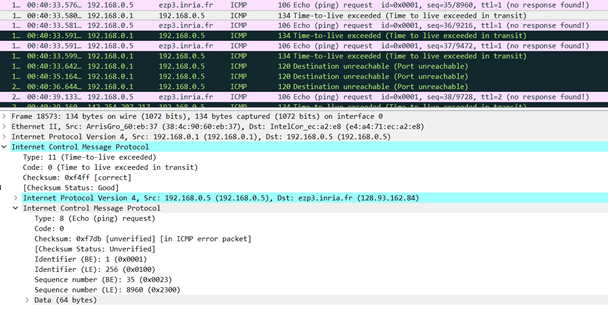
\includegraphics[width=\linewidth]{traceError.png}
	\caption{Captured ICMP Echo Request during Traceroute}
	\label{fig:traceError}
\end{figure}

\section{Lab 4: The Dynamic Host Configuration Protocol}

 Lab 4 addresses the Dynamic Host Control (DHCP) protocol. Unlike MAC Addresses, hosts are not built with a predetermined IP address. When a new host is connected to a network, it must be assigned an IP address. A network administrator could manually assign IP addresses to each host, but such a task would range from time consuming to borderline impossible depending on the size and properties of a network. Instead, DHCP is used to allow flexible, reliable, and automated assignment of IP addresses. Each network must have a DHCP server, which assigns and manages IP addresses for every host in the network \cite{tanenbaum}. To explore the protocol, we will use the {\tt ipconfig/release} command in Windows to release our current IP address, then use {\tt ipconfig/renew} to request a new IP address from the DHCP server. Captured DHCP packets from that process can be viewed in Wireshark to gain insight into the DHCP process.

It is important to understand how hosts and DHCP servers can communicate prior to an IP address for the host being established. All messages during the DHCP assignment process are sent over UDP, with messages to the DHCP server sent on port 67, and messages to the host sent on port 68 \cite{dhcp}. When a new host wants to request an IP address, it sends a DHCP Discover message to the local broadcast address, {\tt 255.255.255.255}. As seen below, the requesting host's MAC address is used for identification. Other hosts on the network will receive the same messages from the DHCP server, but will ignore them due to the unique MAC address. Additionally, the requesting host can request its last known IP address from the DHCP server, which the DHCP server can assign if the address is available.\\

\begin{figure}[h!]

	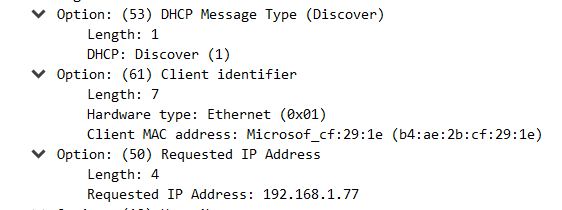
\includegraphics[width=\linewidth]{DHCPDiscovery.png}
	\caption{DHCP Discover Message Options}
	\label{fig:dhcpCap1}
\end{figure}
 
 After receiving a DHCP Discover message, the DHCP server responds with a DHCP Offer message, which contains an IP address for the host, as well as the IP address of the local gateway router. The host then responds with a DHCP Request message, letting the server know that it accepts the offered IP information. The server responds with a DHCP ACK message, which is the first message in the process that is sent using the host's newly assigned IP address, as seen below. \\
 
 \begin{figure}[h!]

	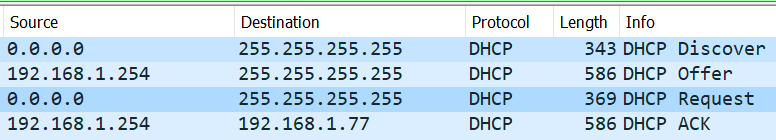
\includegraphics[width=\linewidth]{dhcpprocess.png}
	\caption{4-Step DHCP Assignment Process}
	\label{fig:dhcpCap2}
\end{figure}

 When the DHCP server assigns IP addresses, it includes an expiration time for those addresses. Hosts that want to continue using the IP address can renew the lease on the IP address the same way someone renting an apartment can renew the lease when their current lease is expiring. In our captured messages, the DHCP server leases the IP addresses for 1 day, and allows the renewal of the releases after 12 hours. The leasing and renewal of IP addresses allows the DHCP server to maintain the IP addresses of a network without wasting IP addresses on hosts that are no longer active.
 
 From a security perspective, it is important to remember that the DHCP service does not use any authentication. If a malicious DHCP server is placed in a network, a race condition between the legitimate and malicious servers will occur. When a host requests or renews an IP address, whichever server responds first will be treated as the legitimate server, while the second server's messages will be ignored. If the malicious server wins the race condition, it can provide IP information that can serve as a stepping stone to a wide array of powerful man-in-the-middle attacks.
 
  On the passive side, the malicious actor could provide a host with a malicious gateway router, which would allow the attacker to view the network activity of any hosts associated with the rogue DHCP server. Another more active option would be to provide the host with a malicious Domain Name System (DNS) server.  In short, DNS servers translate a website domain name to the IP address of the name. Using a malicious DNS server, an attacker could redirect a host to a clone of a requested website, including online shopping, email, and banking websites. Unsuspecting users would log in at the fake website, providing the attacker with usernames and passwords. While these examples demonstrate a higher level of sophistication, a rogue DHCP server can serve as the starting point to many of these attacks.\\
 
\section{Lab 5: The User Datagram Protocol}

 The purpose of this lab is to get us acquainted with the functionalities of the User Datagram Protocol (UDP) and its packet contents. This is achieved by capturing  UDP packets sent out by a source machine while browsing the internet. Applications that use UDP transmissions are normally real-time applications such as audio/voice, multimedia streaming, or applications where the loss of packets is permitted and reliability is not the primary concern, such as tunneling and online gaming. Similarly, while browsing the internet for videos or streaming music, there is transmission of UDP packets between the host machine and the destination machine \cite{tanenbaum}
 
 Figure \ref{fig:udpCapture} shows a Wireshark trace of captured UDP packets which were sent out during a DNS query. As shown in the figure, a UDP packet header consists of the following fields: Source Port, Destination Port, Length, and Checksum. The length of a UDP header is 8 bytes, and each of the individual field is 2 bytes in length. Source and Destination port fields contain the port numbers used on the source machine and the destination machine, respectively. The value of the Length field denotes the length of the UDP header plus the encapsulated data. The maximum number of bytes that can be included in a UDP payload is limited by the size of the length field, at most 65,527 bytes in length. The largest possible source and destination port numbers are also limited by their size in the header field and is also equal to 65,535. Since UDP is a transport layer protocol, the segment is encapsulated in the IP datagram. The protocol identifier number that reflects a UDP packet in the IP datagram is 17. \\

\begin{figure}[h!]
	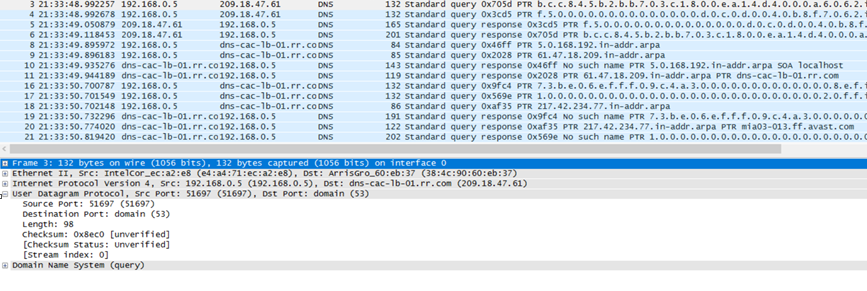
\includegraphics[width=\linewidth]{udpCapture.png}
	\caption{Captured UDP packets}
	\label{fig:udpCapture}
\end{figure}

 UDP is generally meant for unreliable delivery, but it does has a checksum field. The checksum field is optional and services which have better provisions for reliability do not make use of the UDP checksum. Some services such as BOOTP, however, make use of the UDP checksum as their only form of reliability. A UDP checksum, similar to a TCP checksum, is calculated over the UDP header, a pseudo-header, and the data field. The pseudo-header contains the IP source address, IP destination address, protocol number (padded with a zero byte), and the UDP length. This violates the layering principle as the UDP being a layer 4 protocol uses information stored in the layer 3 IP protocol. The checksum is calculated as one's complement of one's complement sum of 16-bit words. \\
 
\section{Lab 6: The Transport Control Protocol}

 While UDP serves some important functions, many applications require a reliable, sequenced byte stream that a connectionless protocol simply can't provide. The Transport Control Protocol (TCP) is a connection-oriented protocol that provides that required reliability, and as a result has become the dominant protocol in the transport layer. In order to investigate the details of TCP, we will upload a text file consisting of Lewis Carroll's \textit{Alice's Adventures in Wonderland} to a website, and analyze captured packets from that upload.
 
 Before addressing the specific TCP packets from our upload, we must quickly review some components of the TCP header. The relevant fields for our purposes are the source port, destination port, sequence number, acknowledgment number, and flag bits. Ports allow hosts to distinguish data meant for different applications. Ports 0 through 1024, called well-known ports, are reserved for standard services. For example, port 80 is used for HTTP, while port 443 is used for HTTPS. Other applications can pick higher, unreserved port numbers for their specific use \cite{tanenbaum}. In our captured upload, the sender is using port 54208, and sending the TCP segments to port 80, as seen in Figure \ref{fig:TCPPortNumbers}.\\
 
  \begin{figure}[h!]
	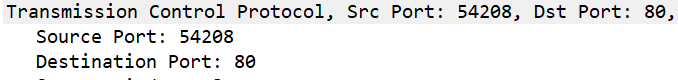
\includegraphics[width=\linewidth]{portnumbers.png}
	\caption{Source and Destination Port Numbers }
	\label{fig:TCPPortNumbers}
\end{figure}

 There are nine flag bits in the TCP header. Setting one or more flag bits provides information on how the TCP segment should be handled. The three-way handshake that begins our data upload is a great example of how TCP flags are used. Because TCP is a full duplex, connection-oriented protocol, it must establish a connection between the two hosts before attempting to send any application data. A host initiates the handshake by sending a packet with the SYN flag set. The receiving host responds with a packet where both SYN and ACK flags are set. The initiating host responds with an ACK, and the connection is ready for the transmission of application data. Figure \ref{fig:threewayhandshake} shows the three-way handshake that established the connection in this lab.\\
 
    \begin{figure}[h!]
	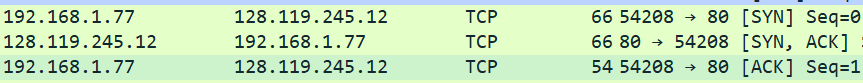
\includegraphics[width=\linewidth]{threewayhandshake.png}
	\caption{Three-way Handshake Prior to File Upload}
	\label{fig:threewayhandshake}
\end{figure}
 
 When considering the sequence and acknowledgement numbers of a TCP segment, it is important to remember that each individual byte is given a sequence number. In our captured packets, we see that our uploaded text file is split into multiple packets due to its large size. In Figure \ref{fig:tcpsequence} we see that each packet includes 1460 bytes of data, the sequence number of each packet is 1460 more than the previous one.\\
 
\begin{figure}[h!]
	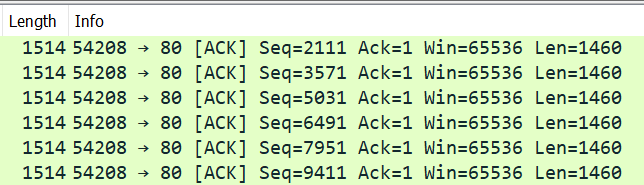
\includegraphics[width=\linewidth]{tcpsequence.png}
	\caption{Sequence Numbers of Uploading Packets Increasing By Data Length}
	\label{fig:tcpsequence}
	\end{figure}
	
 Because TCP uses a sliding window protocol, our uploading host continues to send new data even though previous segments have not yet been acknowledged by the receiver. In figure \ref{fig:tcpack} we see some of the first acknowledgement messages from the receiver begin to arrive, while we continue to send new data. Each acknowledgement number acts as an acknowledgement for all sequence numbers equal to or less than the acknowledgement number, ensuring that each byte is individually accounted for. In our captured upload, no data needed to be resent, indicated by no sequence number being sent twice.\\
 
 \begin{figure}[h!]
 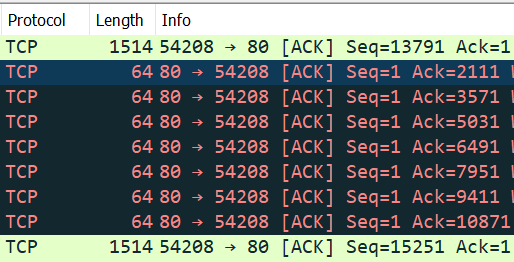
\includegraphics[width=\linewidth]{tcpack.png}
 \caption{Acknowledgment Numbers Begin to Arrive}
 \label{fig:tcpack}
 \end{figure}
 
  Occasionally we see acknowledgement messages for every other packet sent. This is known as delayed acknowledgement, and is allowed under RFC 1122 \cite{tcp}. Because acknowledgement numbers are cumulative, it is possible to acknowledge multiple packets with a single response. Figure \ref{fig:delayedack} shows one example of a delayed acknowledgement from our capture. Under the RFC, delayed acknowledgement messages should never cover more than two received packets. \\
 
  \begin{figure}[h!]
 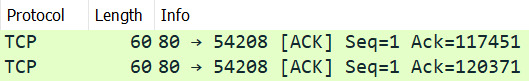
\includegraphics[width=\linewidth]{delayedack.png}
 \caption{A Delayed Acknowledgement Message Covering Two Packets (2920 bytes) of Data}
 \label{fig:delayedack}
 \end{figure} 
 
 The size of the window used for the connection is limited by the buffer size of the receiving host. This buffer size is initially determined during the three-way handshake, and can be readjusted throughout the connection process. This ensures that network congestion does not cause any packets to be lost. One way TCP attempts to find the optimum throughput is by increasing the window size every time a good acknowledgement is received. In Figure \ref{fig:increasingwindow}, listed in the appendix, we see that our uploaded packets were not sent as a constant stream. Instead, the packets were sent in smaller batches corresponding to the window size. As acknowledgments were received, the batches increased in size.  Also shown in the appendix, we see how the average throughput, measured in bits per second, steadily increases as the window size increases. In this particular lab, the window size and throughput continued to increase, and no additional congestion avoidance measures were taken. A larger file upload would provide more information on the maximum throughput the connection could achieve in practice. 
   
 As a quick note, it is important to recognize that many of the tools that allow TCP to be a flexible and efficient protocol can be used against it by malicious users. While the unreserved port numbers above 1024 provide flexibility for applications, malicious actors can also take advantage of the ambiguity of high port numbers. When attackers create a connection between an infected host and the attacker's machine, they often pick a random high port for the connection, making it difficult to distinguish a legitimate connection from a malicious one. Running a {\tt netstat} command on Windows gives us a picture of all active connections and their port numbers, and helps us appreciate the benefit and risk of using dynamically assigned high port numbers.

 The automated responses of hosts to various TCP messages can also be used by malicious actors. Network mapping tools such as Nmap take advantage of this to identify a wide array of useful information, including hosts within a network, open ports, and operating system information \cite{nmap}. A simple Nmap scan run on the author's personal network shows how TCP can be a powerful tool to both network administrators and malicious actors alike. As seen in Figure \ref{fig:nmapscan}, The scan quickly identified a number of the author's devices on the network, including a printer and a wireless speaker. Additionally, the scan identified specific ports and services open on the printer, which could be used by an attacker to deliver malicious payloads targeting vulnerabilities in those specific services.\footnote{This scan was run by the author, limited to the author's personal network, with the author's permission. Active port scanning should always be conducted with the explicit permission of the network owner.}
 
    \begin{figure}[h!]
	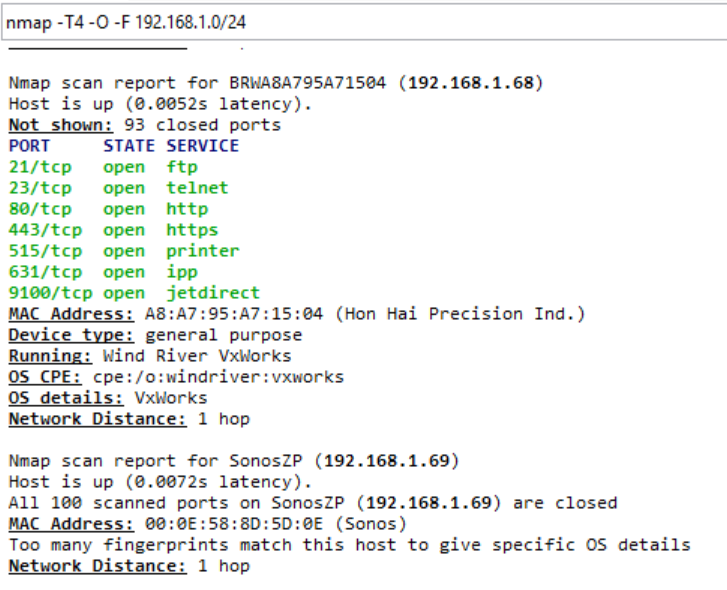
\includegraphics[width=\linewidth]{nmapscan.png}
	\caption{Automated responses to specific TCP packets provide information regarding the author's printer}
	\label{fig:nmapscan}
\end{figure}
 
\section{Conclusion}

 Individually, each lab provided a number insights into some of the most important protocols used in modern computer networking. Taken as a whole, the labs gave us a picture of how multiple protocols, working from MAC addresses at the link layer up to DHCP at the application layer, work together to transfer information. Additionally, the labs served as an excellent introduction to Wireshark, which provided a great deal of information on protocols across multiple layers. We also saw how helpful aspects of protocols and tools can be co-opted by malicious actors. As with most technology, the morality of its use is determined by the intent of the user, not the technology itself.
 
 None of the labs serve as a comprehensive exploration of any one protocol. Each protocol and tool covered in this report can be explored in much greater detail. There are also a wide variety of protocols and tools used in computer networking that were not covered by these labs, but are nonetheless important to the overall goal of communication.\\
 
\bibliographystyle{IEEE} 
\begin{thebibliography}{1}

\bibitem{wireshark}
"Wireshark: About." 2017, https://wireshark.org/

\bibitem{tanenbaum}
Andrew S. Tanenbaum and David J. Wetherall
\textit{Computer Networks, 5th Edition}. Prentice Hall, Boston, 2011

\bibitem{dhcp}
[RFC2131] Droms, R., "Dynamic Host Configuration Protocol", RFC 2131, DOI 10.17487/RFC2131, March 1997, http://www.rfc-editor.org/info/rfc2131.

\bibitem{tcp}
[RFC1122] Braden, R., Ed., "Requirements for Internet Hosts - Communication Layers", STD 3, RFC 1122, DOI 10.17487/RFC1122, October 1989, http://www.rfc-editor.org/info/rfc1122.

\bibitem{nmap}
"Nmap: Introduction." 2017, https://nmap.org/

\end{thebibliography}

\newpage

\begin{appendix}

\subsection{Lab 1 Figures}
 Figure \ref{fig:httpok} shows the HTTP OK message that was received as a response to the HTTP GET message sent out by our machine to the \textit{gaia.cs.umass.edu} server.
\begin{figure}[h!]
	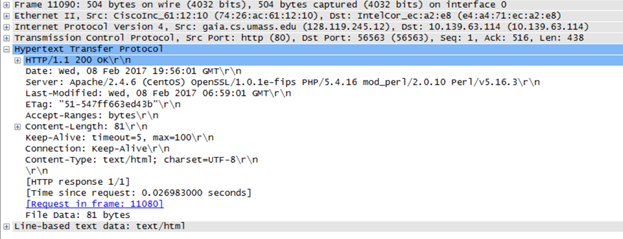
\includegraphics[width=\linewidth]{HTTPOK.PNG}
	\caption{HTTP OK reply received}
    \label{fig:httpok}
\end{figure}

\subsection{Lab 3 Figures}
 Figure \ref{fig:cmdping} shows the command line interface of a windows machine executing the Ping program. Ten ping probes are sent as mentioned in the command. A captured Ping Reply message is shown in figure \ref{fig:pingreply}. As can be seen from the figure, the type field and the code field of a Ping Reply message are 0 indicating that they are the Ping reply messages. 
 
\begin{figure}[h!]
	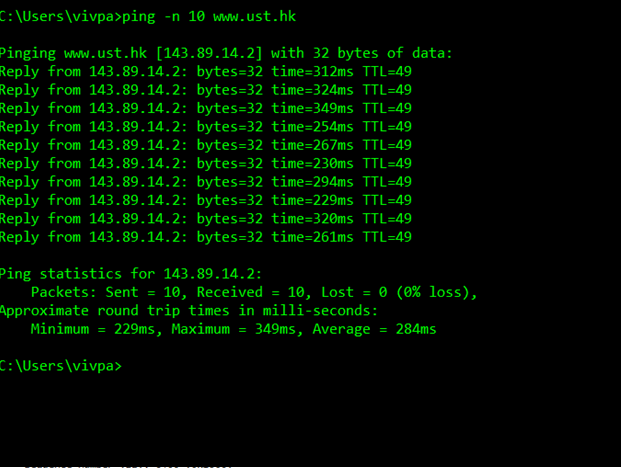
\includegraphics[width=\linewidth]{Ping.png}
	\caption{Ping message sent to www.ust.hk}
    \label{fig:cmdping}
\end{figure}

\begin{figure}[h!]
	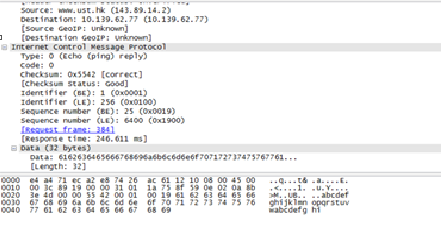
\includegraphics[width=\linewidth]{PINGREPLY.PNG}
	\caption{Captured ICMP Ping Reply Message}
    \label{fig:pingreply}
\end{figure}

Figure. \ref{fig:cmdTrace} shows the command line interface of a Windows machine executing a Traceroute program. As we can see, the destination is 20 hops away from our host machine. As mentioned before, a host machine sends a traceroute probe in the increasing values of TTL field, starting from one. Figure. \ref{fig:icmperror} shows a TTL exceeded error message that was sent back because the traceroute probe didn't make it to the destination before the TTL value reached one. 

\begin{figure}[h!]
	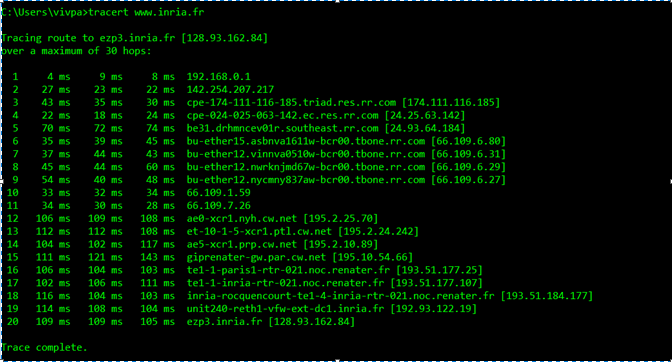
\includegraphics[width=\linewidth]{tracert.png}
	\caption{Traceroute sent to INRIA}
    \label{fig:cmdTrace}
\end{figure}

\begin{figure}[h!]
	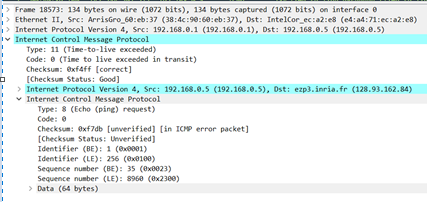
\includegraphics[width=\linewidth]{ICMPError.PNG}
	\caption{ICMP Time-To-Live-Exceeded error message}
    \label{fig:icmperror}
\end{figure}

The delay for the traceroute probe depends on the length of the link the probe spans. So, for a transoceanic link, the delay increases considerable, as shown in figure. \ref{fig:transoceanic}.

\begin{figure}[h!]
	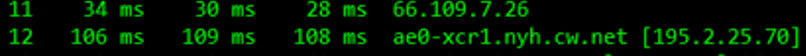
\includegraphics[width=\linewidth]{transoceanic.png}
	\caption{TransOceanic link during Traceroute Program}
    \label{fig:transoceanic}
\end{figure}

\subsection{Lab 5 Figures}
The type of protocol sent out during a transmission can be found out by checking the protocol type field in the IP header. As shown in figure. \ref{fig:udp_pro_type}, the datagram of the IP packet contains a UDP segment, since the protocol type field has a value 17.  

\begin{figure}[h!]
	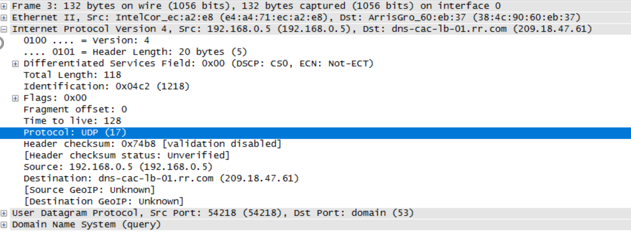
\includegraphics[width=\linewidth]{udp_pro_type.PNG}
	\caption{UDP protocol type as seen in IP header}
	\label{fig:udp_pro_type}
\end{figure}


\subsection{Lab 6 Figures}

\begin{figure}[h!]
	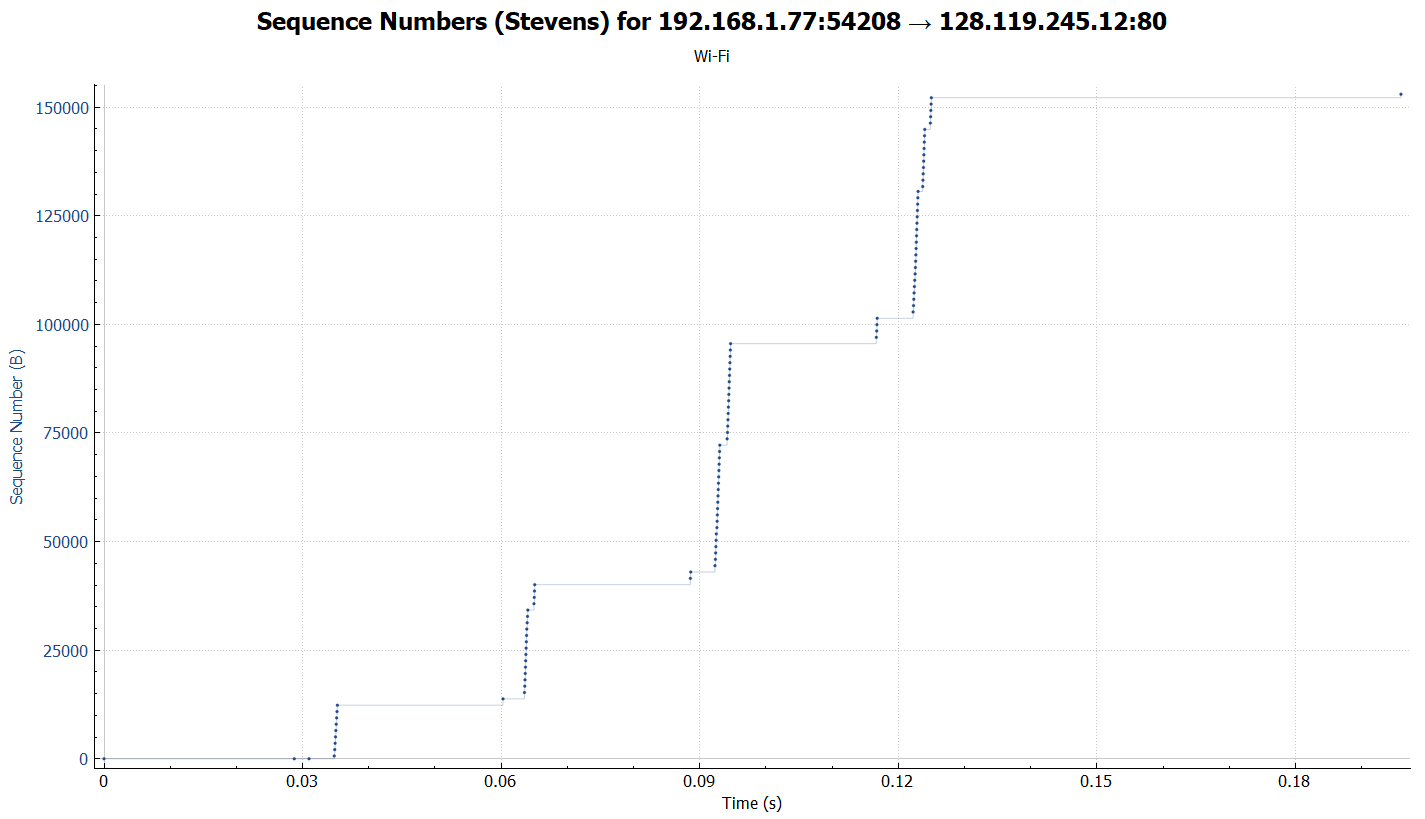
\includegraphics[width=\linewidth]{increasingwindow.png}
	\caption{Window Size Increasing as Acknowledgments Arrive}
	\label{fig:increasingwindow}
\end{figure}

\begin{figure}[h!]
 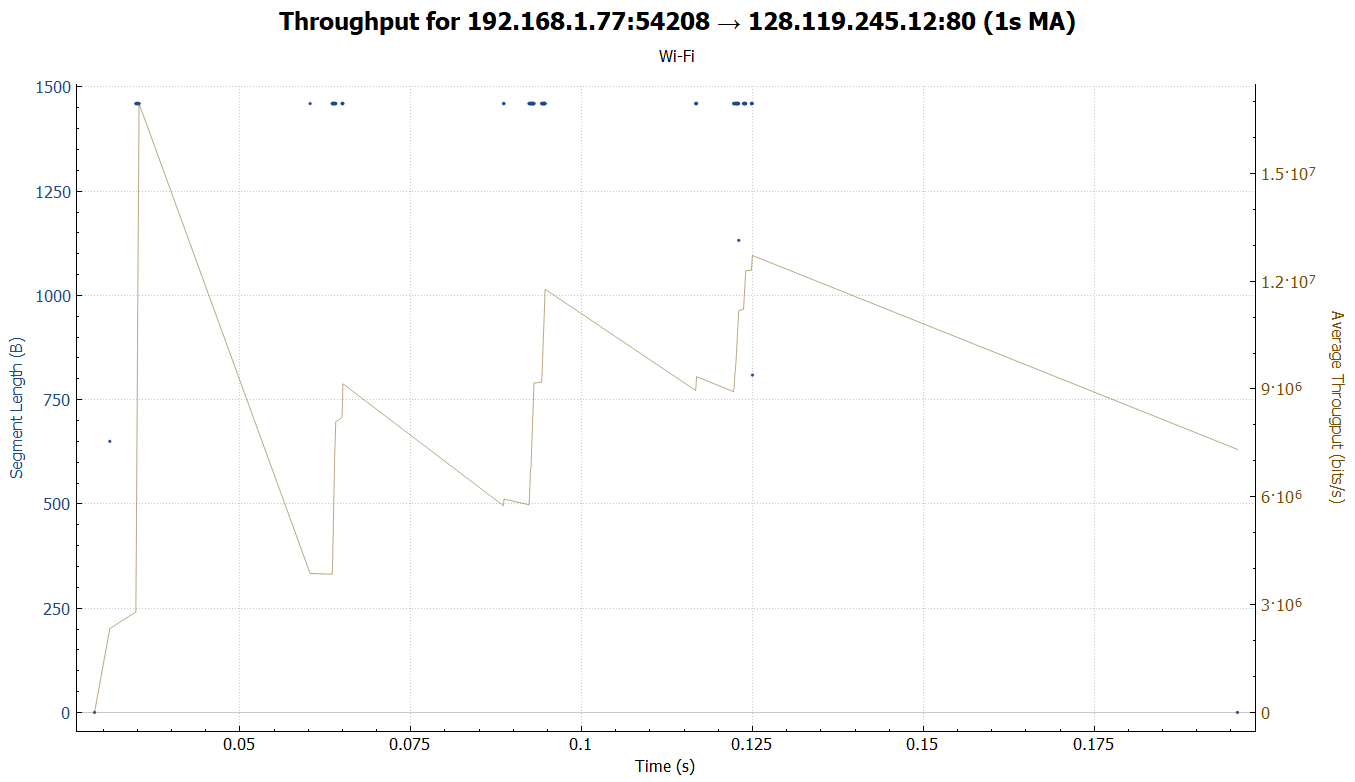
\includegraphics[width=\linewidth]{tcpthroughput.png}
 	\caption{Average throughput of the file upload increases as the window size increases}
    \end{figure}

\end{appendix}

\end{document}